\section{Rotational Mechanics}

\subsection{torque}


we define torque of a force as product of force and its lever arm: $\boxed{\tau = F r}$

where lever arm $r$ is perpendicular distance from line of action to pivot

torque acting on a rigid body produces turning effects

torque is a vector quantity\footnote{More formally, torque is defined as $\vec{\tau} = \vec{r} \times \vec{F}$.}, which can act in clockwise or counter-clockwise direction


\subsubsection*{torque due to weight}

for a body of mass $M$, weight acts on every small constituent piece $\Delta m_i$, where $M=\sum_i \Delta m_i$

net torque due to weight is $\tau—_\text{body} = \sum_i \tau_i = \left(\sum_i \Delta m_i g r_i\right) = \left(\sum_i \Delta m_i r_i\right) g$\footnote{I am a bit sloppy here. We should use the lever arm distance from a chosen pivot, or we should write $\vec{\tau}_\text{body}\ = \sum_i \Delta m_i \vec{r}_i \times \vec{g}$. But as long as we keep that in mind, the results that follow are valid.}

we introduce centre of mass, such that $\boxed{\left(\sum_i \Delta m_i r_i\right) = \left(\sum_i \Delta m_i\right) r_\text{cm}}$, or $\left(\sum_i \Delta m_i r_i\right) = M r_\text{cm}$

$r_\text{cm} = \frac{\sum_i \Delta m_i r_i}{\sum_i \Delta m_i}$ gives position of centre of mass from a chosen origin

taking continuum limit: $\Delta m_i \to \dd m \RA \boxed{r_\text{cm} = \frac{\int r \dd m}{\int \dd m}}$

$r_\text{cm}$ can be thought as the weighted average of position vector $r_i$'s

net torque due to weight can be therefore computed as: $\boxed{\tau_\text{body} = Mgr_\text{cm}}$

entire weight on rigid body can be considered to act at centre of mass

\example{A uniform rod $AB$ has mass $4m$ and length $L$. A particle of mass $m$ is attached at $A$ and another particle of mass $2m$ is attached at $B$. The system is allowed to rotate about a horizontal axis perpendicular to the rod and through $A$. (a) Find the position of the centre of mass. (b) When the system is displaced by an angle $\theta$ from the downward vertical, what is the torque by gravity?} \label{ex-lever}

\begin{figure}[htp]
	\centering
	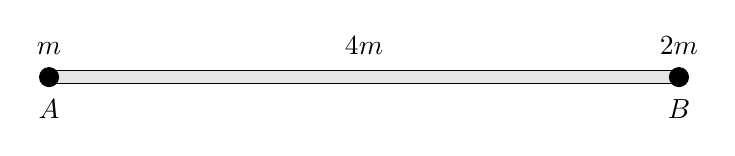
\begin{tikzpicture}[scale=0.8]
	\draw[fill=gray!20] (-5,-0.1) rectangle (5,0.1);
	\draw[fill] (-5,0) circle(0.15);
	\draw[fill] (5,0) circle(0.15);
	\node[below] at (-5,-0.2) {$A$};
	\node[below] at (5,-0.2) {$B$};
	\node[above] at (-5,0.2) {$m$};
	\node[above] at (5,0.2) {$2m$};
	\node[above] at (0,0.2) {$4m$};
	\end{tikzpicture}
	
	Example \ref{ex-lever}
\end{figure}

{
	
\centering
	
$(m\cdot 0 + 2m\cdot L + 4m \cdot \frac{1}{2}L) = (m+2m+4m)x_\text{cm} \RA x_\text{cm} = \frac{4}{7}L$

}

centre of mass is at $\frac{4}{7}L$ from $A$ (near mid-point of $AB$ but slightly closer to the heavier end)

when suspended, torque by gravity can be found using $r_\text{cm}$

{
	
\centering

$\tau = Mgr_\text{cm} \RA \tau_\text{body} = 7mg\cdot \frac{4}{7}L\sin\theta = 4mgL\sin\theta$

}

(or by summing up torques of each part: $\tau = 0 + 2mg\cdot L\sin\theta + 4mg\cdot\frac{1}{2}L\sin\theta = 4mgL\sin\theta$) \eoe

\subsection{moment of inertia}

\subsubsection{moment of inertia: the motivation}\label{moim}

a rigid body means an object never undergoes change in shape

let's think of it a system of many small pieces of mass $\Delta m_i$

distance between any two pieces remains the same whatever you do

if each piece is acted by some resultant force $F_i = \Delta m_i a_i$

torque on this piece: $\tau_i = F_i r_i = (\Delta m_i a_i) r_i = (r_i^2 \Delta m_i)\frac{a_i}{r_i}$

recall $\alpha = \frac{a_i}{r_i}$ gives the angular acceleration

torque on one individual piece: $ \tau_i =  r_i^2 \Delta m_i  \alpha $

to find out what resultant torque does, sum up for all pieces: $\sum_i \tau_i = \sum_i (r_i^2 \Delta m_i \alpha)$

but angular acceleration is the same throughout a rigid body (rotation as a whole)

so $\alpha$ can be taken out from the summation: $ \sum_i \tau_i = \left(\sum_i r_i^2 \Delta m_i\right) \alpha$

\vspace*{\baselineskip}

we introduce moment of inertia of a rigid body: $\boxed{I = \sum_i r_i^2 \Delta m_i}$

taking continuum limit: $\Delta m_i \to \dd m \RA \boxed{I = \int r^2 \dd m}$

hence we have the equivalent of Newton's $2^\text{nd}$ law: $\boxed{\sum \tau_i = I \alpha}$

this states a resultant torque on a rigid body produces angular acceleration that is inversely proportional to its moment of inertia (compare with this: a resultant force produces linear acceleration that is inversely proportional to object's inertia mass)

moment of inertia describes how a rigid body resists change in rotational motion when acted by a resultant torque, hence plays an important role in rotational mechanics

we will next study how to compute moment of inertia for different bodies

\subsubsection{moment of inertia: some useful results}

we here present the moment of inertia of some regular objects 

note that all $I$'s listed below are about a perpendicular axis through centre

\begin{center}
	{\renewcommand{\arraystretch}{1.2}
	\renewcommand{\tabcolsep}{0.2cm}
	\begin{tabular}{|cc|c|}
		\hline
		\multicolumn{2}{|c|}{uniform object with mass $m$} & moment of inertia \\
		\hline
		ring & radius $R$ & $I=mR^2$ \\ \hline
		disc/solid cylinder & radius $R$ & $I=\frac{1}{2}mR^2$ \\ \hline
		thin rod & length $2L$ & $I=\frac{1}{3}mL^2$ \\ \hline	
		rectangular lamina & sides $2a$, $2b$ & $I=\frac{1}{3}m(a+b)^2$ \\ \hline
		solid sphere & radius $R$ & $I=\frac{2}{5}mR^2$ \\ \hline
		spherical shell & radius $R$ & $I=\frac{2}{3}mR^2$ \\ \hline
	\end{tabular}}
\end{center}

all of these can be shown using the defining equation: $I = \sum_i r_i^2 \Delta m_i$, or $I = \int r^2 \dd m$

we show the proofs for a few items on the list, the rest will be left as exercise for the reader \footnote{Spoiler alert: this left-as-exercise nonsense occurs whenever the author simply does not want to typeset more equations or diagrams.}

\subsubsection*{point mass}

consider a particle of mass $m$ rotates about an axis at distance $R$

simply recall defining equation: $I_\text{pt}=mR^2$

\subsubsection*{uniform ring}

\begin{figure}[htp]
	\centering
	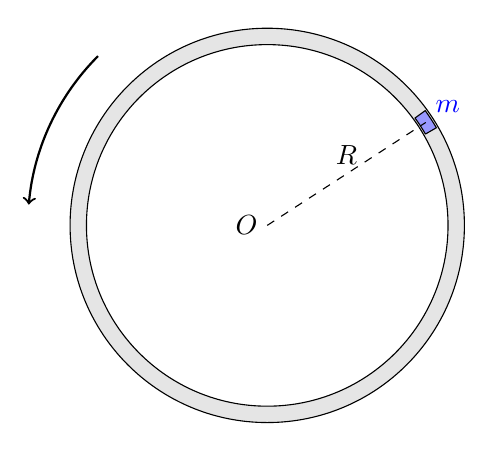
\begin{tikzpicture}[scale=0.8]
	\draw[line width=6,gray!20] (0,0) circle(3);
	\draw (0,0) circle(3.13);
	\draw (0,0) circle(2.87);
	\draw[fill=blue!40] (30:2.9) -- ++ (30:0.2) arc(30:36:3.1) --++ (36:-0.2) arc(36:30:2.9);
	\draw[dashed] (0,0)node[left]{$O$} -- (33:3) node[midway,above]{$R$} node[above right,blue]{$\dd m$};
	\draw[thick, ->] (135:3.8) arc(135:175:3.8);
	\end{tikzpicture}
	
	uniform ring of radius $R$
\end{figure}

a uniform ring of mass $m$ rotates about perpendicular axis through its centre $O$

any piece $\Delta m$ is of same distance to $O$, which is radius $R$ of the ring

so $I_\text{ring} = \int r^2 \dd m = R^2 \int \dd m \RA \boxed{I_\text{ring} = mR^2}$


\subsubsection*{uniform disc}

\begin{figure}[htp]
	\centering
	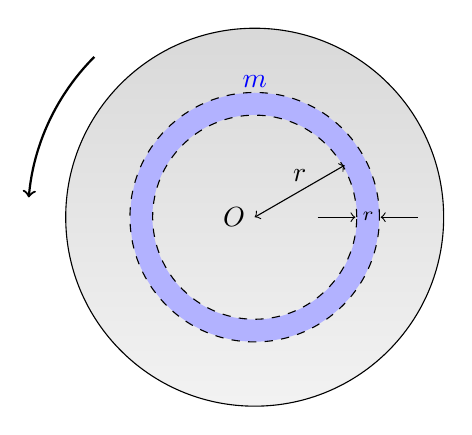
\begin{tikzpicture}[scale=0.8]
	\shadedraw[top color=gray!30,bottom color=gray!10, draw=black] (0,0) circle(3);
	\draw[line width=8,blue!30] (0,0) circle(1.8);
	\draw[dashed] (0,0) circle(1.98);
	\draw[dashed] (0,0) circle(1.62);
	\draw[<->] (0,0)node[left]{$O$} -- (30:1.65) node[midway,above]{$r$};
	\draw[->] (1,0) -- (1.6,0);
	\draw[<-] (2,0) -- (2.6,0);
	\node at (1.8,0.02) {{\scriptsize $\dd r$}};
	\node[above,blue] at (0,1.9) {$\dd m$};
	\draw[thick, ->] (135:3.6) arc(135:175:3.6);
	\end{tikzpicture}
	
	uniform disc of radius $R$
\end{figure}

a uniform disc of mass $m$ rotates about perpendicular axis through its centre $O$

consider a narrow ring of radius $r$ and thickness $\dd r$ about $O$

area of this ring is: $\dd A = 2 \pi r \dd r$

its mass is therefore: $\dd m = \frac{2 \pi r \dd r}{\pi R^2}\cdot m = \frac{2mr}{R^2}\dd r$

so $I_\text{disc} = \int r^2 \dd m = \int_0^R r^2 \frac{2mr}{R^2}\dd r = \frac{2m}{R^2}\int_0^R r^3 \dd r = \frac{2m}{R^2} \times \frac{R^4}{4}\RA \boxed{I_\text{disc} = \frac{1}{2}mR^2}$

\subsubsection*{uniform rod}

\begin{figure}[htp]
	\centering
	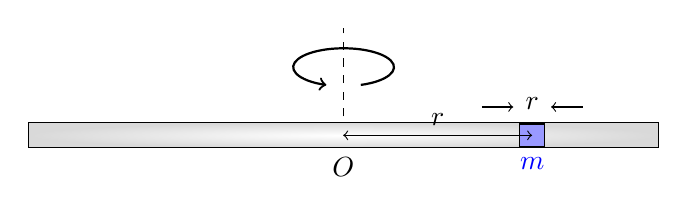
\begin{tikzpicture}[scale=0.8]
	\shadedraw[inner color=white,outer color=gray!30, draw=black] (-5,-0.2) rectangle (5,0.2);
	\draw[fill=blue!40] (2.8,-0.18) rectangle (3.2,0.18);
	\draw[<->] (0,0) -- (3,0) node[midway,above]{$r$};
	\draw[->] (2.2,0.45) -- (2.7,0.45);
	\draw[<-] (3.3,0.45) -- (3.8,0.45);
	\node at (3,0.5) {$\dd r$};
	\node[below] at (0,-0.2) {$O$};
	\node[below,blue] at (3,-0.2) {$\dd m$};
	\draw[thick, ->] (0.28,0.8) arc(-70:250:0.8 and 0.3);
	\draw[dashed] (0,0.3) --++ (0,1.4);
	\end{tikzpicture}
	
	uniform rod of length $2L$
\end{figure}

a uniform rod of mass $m$ rotates about perpendicular axis through its centre $O$

consider a narrow piece of thickness $ \dd r$ at distance $r$ from $O$

mass of this piece: $\dd m = \frac{\dd r}{2L}\cdot m = \frac{m}{2L}\dd r$

so $I_\text{rod} = \int r^2 \dd m = \int_{-L}^L r^2 \frac{m}{2L}\dd r = \frac{m}{2L} \int_{-L}^L r^2 \dd r = \frac{m}{2L} \times \frac{2L^3}{3}\RA \boxed{I_\text{rod} = \frac{1}{3}mL^2}$

\subsubsection{parallel axis theorem}

\noindent\textbf{theorem:} moment of inertia of a rigid body of mass $m$ about any axis can be found from its moment of inertia about a parallel axis through its centre of mass: $\boxed{I_P = I_\text{cm}+ md^2}$, where $d$ is perpendicular distance between the two parallel axes

\begin{figure}[htp]
	\centering
	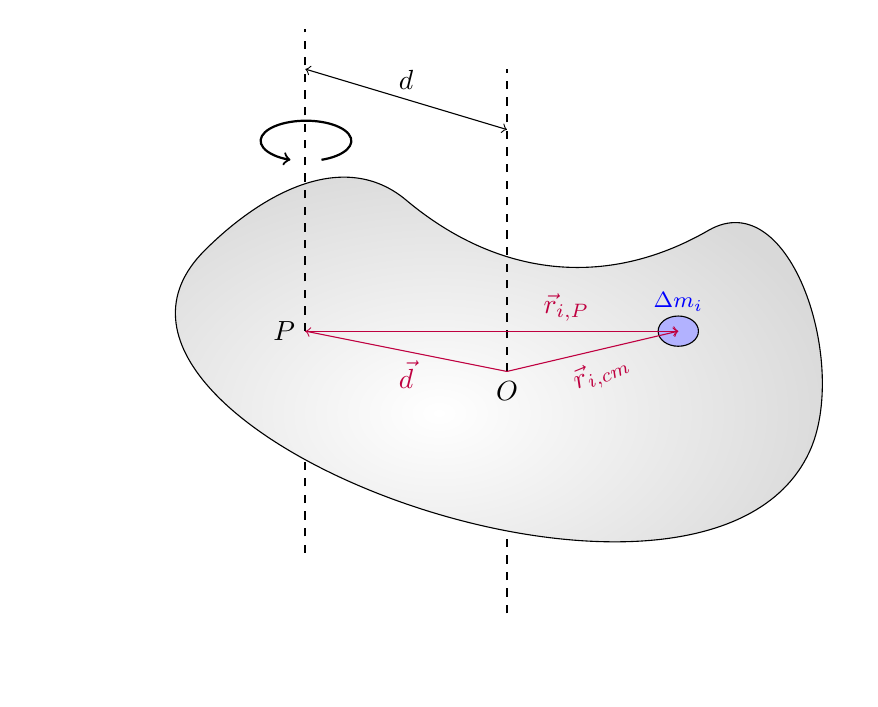
\begin{tikzpicture}[scale=1.28]
	\shadedraw[inner color=white,outer color=gray!30, draw=black] (-2,0) to [out=45,in=140] (0,0.5) to [out=-40,in=210] (3,0.2) to [out=30,in=65] (4,-2) to [out=245,in=225] (-2,0);
	\draw[dashed,thick] (1,-3.6) -- (1,-2.8) (1,-1.2)node[below]{$O$} -- ++(0,3);
	\draw[dashed,thick] (-1,-3) -- (-1,-2.1) (-1,-0.8)node[left]{$P$} -- ++(0,3);
	\draw[<->] (-1,1.8) --++ (2,-0.6) node[above,midway]{$d$};
	\draw[fill=blue!30] (2.7,-0.8) ellipse (0.2 and 0.15);
	\node[blue,above] at (2.7,-0.7) {{\footnotesize $\Delta m_i$}};
	\draw[->,purple] (-1,-0.8) -- (2.7,-0.8) node[above,pos=0.7]{$\vec{r}_{i,P}$};
	\draw[->,purple] (1,-1.2) -- (2.7,-0.8) node[below,pos=0.5,rotate=22.4]{$\vec{r}_{i,\text{cm}}$};
	\draw[<-,purple] (-1,-0.8) -- (1,-1.2) node[below,midway]{$\vec{d}$};
	\draw[thick, ->] (-.84,0.9) arc(-70:250:0.45 and 0.2);
	\end{tikzpicture}
\end{figure}

\vspace*{-\baselineskip}

\noindent\textbf{proof:} $I_P = \sum r_{i,P}^2 \Delta m_i = \sum (\vec{r}_{i,\text{cm}}-\vec{d})^2 \Delta m_i = \sum r_{i,\text{cm}}^2 \Delta m_i + \sum d^2 \Delta m_i - 2\sum \vec{r}_{i,\text{cm}} \cdot \vec{d} \Delta m_i$

first term: $I_\text{cm} = \sum r_{i,\text{cm}}^2 \Delta m_i$, so this is just moment of inertia about centre of mass

second term: $\sum d^2 \Delta m_i = d^2 \sum m_i = md^2$

in last term, we have: $\sum \vec{r}_{i,\text{cm}} \cdot \vec{d} \Delta m_i = \big(\sum \vec{r}_{i,\text{cm}} \Delta m_i \big) \cdot \vec{d}$

notice the term in bracket is related to distance from centre of mass (recall $m\vec{r}_\text{cm} = \sum \Delta m_i \vec{r}_i$)

but here we are evaluating the distance from centre of mass to centre of mass, so it is zero

put everything together, we find: $I_P = I_\text{cm}+ md^2$

\newpage

\vspace*{-1.2\baselineskip}

\example{A system consists of a solid sphere of mass $5m$ and radius $a$, a uniform rod of mass $4m$ and length $3a$ and a particle of mass $2m$. The objects are joined together as shown in the figure below. What is the moment of inertia of this system about an axis through $X$ perpendicular to the rod?} \label{ex-lollipop}

\begin{figure}[ht]
	\centering
	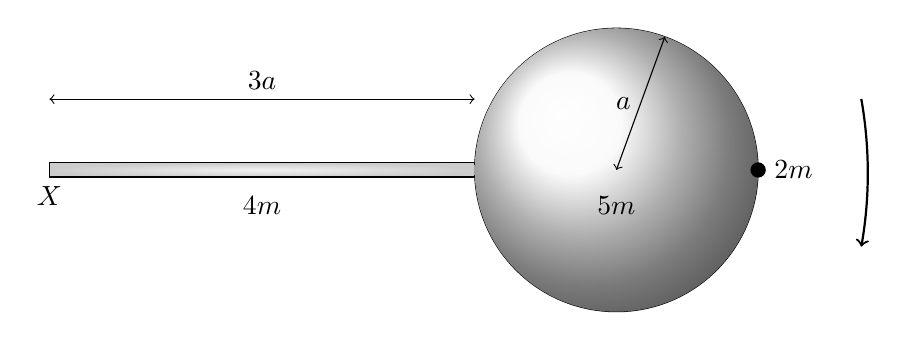
\begin{tikzpicture}[scale=0.9]
	\shadedraw[inner color=gray!10, outer color=gray!40, draw=black] (0,-0.1) node[below]{$X$} rectangle (6,0.1);
	\draw (8,0) circle (2);
	\shade[ball color = gray!5] (8,0) circle (2);
	\draw[fill] (10,0) circle(0.1);
	\draw[<->] (0,1) --++ (6,0) node[midway,above]{$3a$};
	\draw[<->] (8,0) --++ (70:2) node[midway,left]{$a$};
	\node at (3,-0.5) {$4m$};
	\node at (8,-0.5) {$5m$};
	\node at (10.5,0) {$2m$};
	\draw[thick, ->] (5:11.5) arc(10:-10:6);
	\end{tikzpicture}
%	
%	Example \ref{ex-lollipop}
\end{figure}

$I_\text{rod} = \frac{1}{3}\cdot 4m \cdot \left(\frac{3a}{2}\right)^2 + 4m \cdot \left(\frac{3a}{2}\right)^2 = (3+9) ma^2 = 12ma^2$

$I_\text{sphere} = \frac{2}{5}\cdot 5m\cdot a^2 + 5m \cdot(a+3a)^2 = (2+80) ma^2 = 82ma^2$

$I_\text{pt} = 2m \cdot (3a+2a)^2 = 50 ma^2$

$I_\text{sys} = I_\text{rod}  + I_\text{sphere}  + I_\text{pt} = (12+82+50)ma^2 \RA I_\text{sys} = 144ma^2 $ \eoe

\subsubsection{perpendicular axis theorem}

\noindent\textbf{theorem:} given a thin lamina (negligible thickness), its moment of inertia about an axis perpendicular to the plane is equal to the sum of moments of inertia about two perpendicular axes lying within the plane through the same point

suppose the lamina lies within $xy-$plane, then the theorem suggests: $\boxed{I_z = I_x + I_y}$

\begin{figure}[htp]
	\centering
	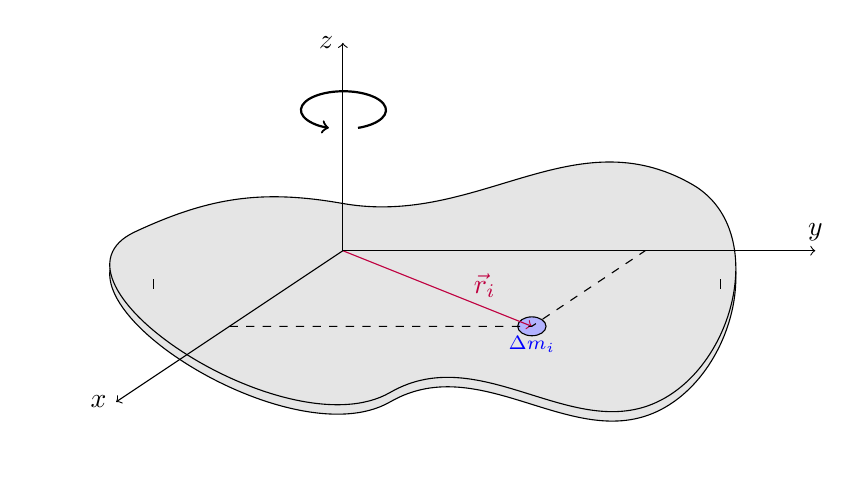
\begin{tikzpicture}[scale=1.2]
	\draw[fill=gray!20] (-3.2,0.4) to [out=25,in=170] (-1,0.7) to [out=-10,in=150] (2.7,0.9) to [out=-30,in=35] (2.5,-1.3) to [out=215,in=30] (-0.5,-1.3) to [out=210,in=205] (-3.2,0.4);
	\draw[fill=gray!20] (-3.2,0.5) to [out=25,in=170] (-1,0.8) to [out=-10,in=150] (2.7,1) to [out=-30,in=35] (2.5,-1.2) to [out=215,in=30] (-0.5,-1.2) to [out=210,in=205] (-3.2,0.5);
	\draw (-3,0) -- (-3,-0.1) (3,0) -- (3,-0.1);
	\draw[fill=blue!30] (1,-0.5) ellipse (0.15 and 0.1);
	\draw[purple,->] (-1,0.3) -- (1,-0.5) node[pos=.75,above]{$\vec{r}_i$};
	\node[blue,below] at (1,-0.5) {{\scriptsize $\Delta m_i$}};
	\draw[->] (-1,0.3) --++ (0,2.2) node[left]{$z$};
	\draw[->] (-1,0.3) --++ (-2.4,-1.6) node[left]{$x$};
	\draw[->] (-1,0.3) --++ (5,0) node[above]{$y$};
	\draw[dashed] (-2.2,-0.5) -- (1,-0.5) -- (2.2,0.3);
	\draw[thick, ->] (-.84,1.6) arc(-70:250:0.45 and 0.2);
	\end{tikzpicture}
\end{figure}

\noindent\textbf{proof:} $I_z = \sum r_{i,z}^2 \Delta m_i = \sum (x_i^2 + y_i^2) \Delta m_i$

$I_x = \sum r_{i,x}^2 \Delta m_i = \sum (y_i^2 + z_i^2) \Delta m_i$, $I_y = \sum r_{i,y}^2 \Delta m_i = \sum (x_i^2 + z_i^2) \Delta m_i$

but all $z_i \approx 0$ for thin lamina, so $I_x = \sum y_i^2 \Delta m_i$, $I_y = \sum x_i^2 \Delta m_i$

it is now obvious to see: $I_z = I_x + I_y$

\example{What is the moment of inertia of a uniform disc of radius $R$ about its diameter?}

\begin{figure}[htp]
	\centering
	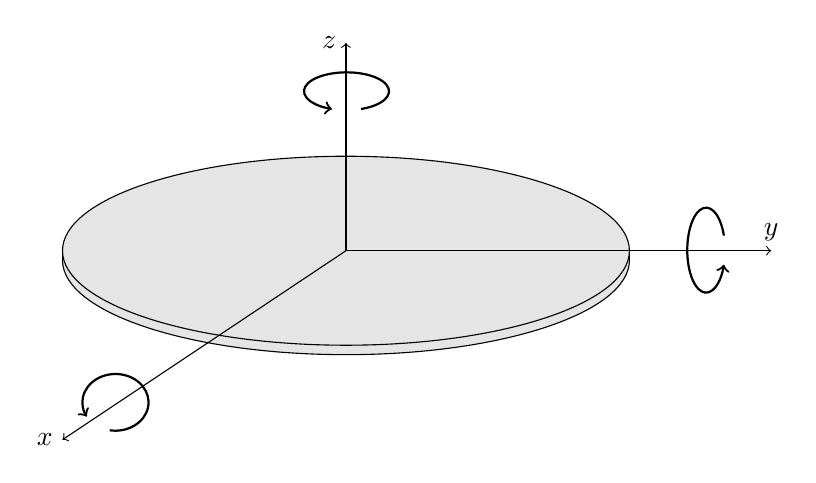
\begin{tikzpicture}[scale=1.2]
	\draw[fill=gray!20] (0,-0.1) ellipse (3 and 1);
	\draw[fill=gray!20] (0,0) ellipse (3 and 1);
	\draw (-3,0) -- (-3,-0.1) (3,0) -- (3,-0.1);
	\draw[->] (0,0) --++ (0,2.2) node[left]{$z$};
	\draw[->] (0,0) --++ (-3,-2) node[left]{$x$};
	\draw[->] (0,0) --++ (4.5,0) node[above]{$y$};
	\draw[thick, ->] (0.16,1.5) arc(-70:250:0.45 and 0.2);
	\draw[thick, ->] (4,0.16) arc(20:340:0.2 and 0.45);
	\draw[thick, ->] (-2.5,-1.9) arc(-100:210:0.35 and 0.3);
	\end{tikzpicture}
\end{figure}

set up perpendicular axes through centre of disc as shown, by theorem: $I_z = I_x + I_y$

but also due to symmetry: $I_x = I_y$, so $I_x = I_y = \frac{1}{2}I_z = \frac{1}{2}\times\frac{1}{2}mR^2 \RA I_x = I_y = \frac{1}{4}mR^2$ \eoe


\subsection{force analysis}

from last section, we have learned how to compute moment of inertia of a rigid body

also from discussion in \S \ref{moim}, we have $\sum \tau_i = I \alpha$, or $\sum \tau_i = I \ddot{\theta}$

now we can predict the motion of a rigid body by applying the equation of motion

\example{A solid cylinder of mass $M$ and radius $R$ rolls down an inclined slope without slipping. What is the acceleration of the body?} \label{ex-rolling}

\begin{figure}[htp]
	\begin{center}
		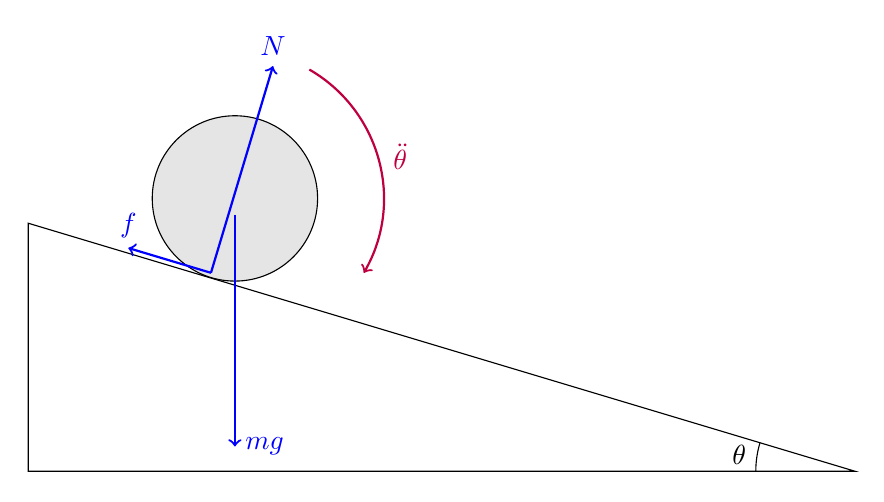
\begin{tikzpicture}[scale=1.05]
		\draw (0,0) --++ (0,3) -- (10,0) -- cycle;
		\draw[fill=gray!20] (2.5,3.3) circle (1);
		\draw[purple,->,thick] (2.5,3.3) ++ (60:1.8) arc(60:-30:1.8);
		\node[purple] at (4.5,3.8) {$\ddot{\theta}$};
		\draw[thick,blue,->] (2.5,3.1) --++ (0,-2.8) node[right]{$mg$};
		\draw[thick,blue,->] (2.21,2.4) --++ (0.75,2.5) node[above]{$N$};
		\draw[thick,blue,->] (2.21,2.4) --++ (-1,0.3) node[above]{$f$};
		\draw (8.8,0) arc(180:163.3:1.2);
		\node at (8.6,0.2) {$\theta$};
		\end{tikzpicture}
		%Example \ref{ex-rolling}
	\end{center}
\end{figure}

resolve along the slope: $mg\sin\theta - f = m\ddot{x}$

torque on cylinder: $f R = \frac{1}{2}mR^2 \cdot \ddot{\theta} \RA f = \frac{1}{2} mR\ddot{\theta}$

together with $\ddot{x}=\ddot{\theta} R$, we have: $mg\sin\theta - \frac{1}{2} mR\cdot \frac{\ddot{x}}{R} = m\ddot{x} \RA \ddot{x}=\frac{2}{3}g\sin\theta$ \eoe

\example{A uniform disc of radius $R$ and mass $M$ is free to rotate without friction about a horizontal
	axis through its centre $O$. A light inextensible string is wound round	the rim of the disc, while a particle of mass $m$ is attached to one end of the string (see diagram). The system is released from rest. Find the angular acceleration of the disc.}\label{ex-rotdisc}

\begin{figure}[htp]
	\begin{center}
		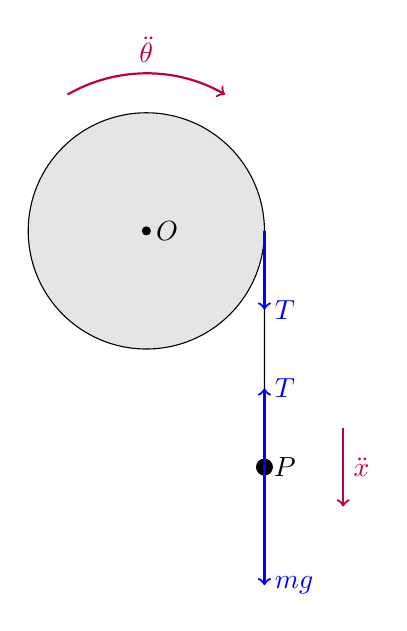
\begin{tikzpicture}[scale=1]
		\draw[fill=gray!20] (0,0)node[right]{$O$} circle (1.5);
		\draw[fill] (0,0) circle(0.05);
		\draw[fill] (1.5,0) -- ++ (0,-3) circle(0.1) node[right]{$P$};
		\draw[thick, ->,purple] (120:2) arc(120:60:2);
		\node[purple] at (0,2.3){$\ddot{\theta}$};
		\draw[thick,purple,->] (2.5,-2.5) --++ (0,-1) node[right,midway]{$\ddot{x}$}; 
		\draw[thick,blue,->] (1.5,-3) --++ (0,-1.5) node[right]{$mg$};
		\draw[thick,blue,->] (1.5,-3) --++ (0,1) node[right]{$T$};
		\draw[thick,blue,->] (1.5,0) --++ (0,-1) node[right]{$T$};
		\end{tikzpicture}
		%Example \ref{ex-rotdisc}
	\end{center}
\end{figure}

for particle: $mg-T=m\ddot{x}$

for disc: $\tau = I \ddot{\theta} \RA T\cdot R = \frac{1}{2}MR^2 \cdot \ddot{\theta} \RA T = \frac{1}{2}MR \cdot \ddot{\theta}$

together with $\ddot{x}=\ddot{\theta} R$, we have: $mg - \frac{1}{2}MR\ddot{\theta} = m\ddot{\theta} R \RA \ddot{\theta} = \frac{2mg}{(2m+M)R}$ \eoe



\subsection{rotational energy}

\subsubsection{rotational kinetic energy}

for a rigid body rotating about some axis, its K.E.: $E_k = \sum_i \frac{1}{2}\Delta m_i v_i^2 = \sum_i \frac{1}{2}\Delta m_i (\omega r_i)^2$

same angular speed $\omega$ throughout, so $E_k = \frac{1}{2} \big(\sum_i r_i^2 \Delta m_i\big) \omega^2$

note that $\sum_i r_i^2 \Delta m_i$ gives the moment of inertia $I$

hence rotational kinetic energy of a rigid body is: $\boxed{E_k = \frac{1}{2} I \omega^2}$

\subsubsection{conservation of mechanical energy}

for rotational motion, conservation of mechanical energy still holds if no energy loss to friction

i.e., change in G.P.E equals change in K.E.

G.P.E. change can be found by comparing initial and final positions of c.o.m.

K.E. change can be computed using new formula $E_k = \frac{1}{2} I \omega^2$

\example{The same rigid-body system as in Example \ref{ex-lollipop} is released from rest from a horizontal position. What is the maximum speed for the particle during the subsequent motion?}

greatest speed when the system becomes downward vertical

increase in K.E. equals loss in G.P.E.: 

{
\centering

$\frac{1}{2}I\omega^2 - 0 = 4mg\cdot \frac{3}{2}a + 5mg\cdot4a+2mg\cdot5a$

$\frac{1}{2}\cdot 144ma^2 \cdot \omega^2 = (6+20+10)mga \RA \omega_\tmax = \sqrt{\frac{g}{2a}}$

}

for the particle: $v_\tmax = \omega_\tmax r = \sqrt{\frac{g}{2a}} \cdot 5a \RA  v_\tmax = \sqrt{\frac{25ga}{2}}$ \eoe

\subsection{small-amplitude oscillations}

when a rigid-body system is displaced from vertical equilibrium by a small angle

it can be shown that the motion is approximately simple harmonic

to do this, the following step-by-step guide is given for reference

\begin{compactenum}
	\item find moment of inertia of the system about the point of suspension
	
	\item when system is displaced by angle $\theta$ from rest position, find resultant torque acting
	
	\item write down equation of motion $\tau = I \ddot{\theta}$, and solve for angular acceleration $\ddot{\theta}$
	
	usually it takes the form $\ddot{\theta} = - \omega^2 \sin\theta$, where $\omega^2$ is some constant with dimension $T^{-2}$
	
	\item apply small-angle approximation ($\sin\theta \approx \theta$ for small $\theta$), one gets $\ddot{\theta} \approx - \omega^2 \theta$
	
	\item identify that this is approximately simple harmonic, period of oscillation can then be found
\end{compactenum}


\example{The same rigid-body system as in Example \ref{ex-lollipop} is slightly displaced from its equilibrium position, show that it performs simple harmonic oscillation provided the angular displacement is small. }

\begin{wrapfigure}{l}{0.3\textwidth}
\begin{center}
	\vspace*{-5pt}
	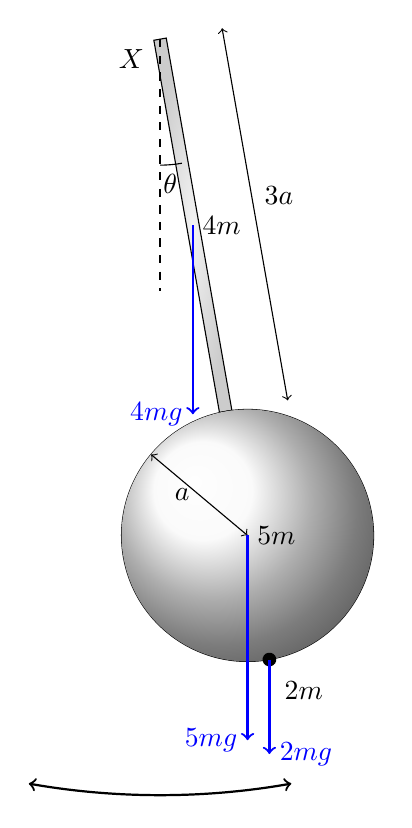
\begin{tikzpicture}[scale=0.8]
	\shadedraw[inner color=gray!10, outer color=gray!40, draw=black,rotate=-80] (0,-0.1) node[below left]{$X$} rectangle (6,0.1);
	\draw[rotate=-80] (8,0) circle (2);
	\shade[ball color = gray!5,rotate=-80] (8,0) circle (2);
	\draw[fill,rotate=-80] (10,0) circle(0.1);
	\draw[<->,rotate=-80] (0,1) --++ (6,0) node[midway,above right]{$3a$};
	\draw[<->,rotate=-80] (8,0) --++ (-140:2) node[midway,left]{$a$};
	\node[right] at (-80:3) {$4m$};
	\node[right] at (-80:8) {$5m$};
	\node[right] at (-80:10.5) {$2m$};
	\draw[thick, <->] (-80:12) arc(-80:-100:12);
	\draw[->,thick,blue] (-80:3) --++ (0,-3) node[left]{$4mg$};
	\draw[->,thick,blue] (-80:8) --++ (0,-3.25) node[left]{$5mg$};
	\draw[->,thick,blue] (-80:10) --++ (0,-1.5) node[right]{$2mg$};
	\draw[dashed] (0,0) -- (0,-4);
	\draw (-80:2) arc(-80:-90:2);
	\node at (-86:2.3) {$\theta$};
\end{tikzpicture}
\end{center}
\vspace*{-15pt}
\end{wrapfigure}

moment of inertia is found to be: $I=144ma^2$

when displaced by $\theta$, magnitude of net torque on system is

{
\centering

$\tau = 4mg\cdot\frac{3}{2}a\sin\theta + 5mg\cdot4a\sin\theta + 2mg\cdot5a\sin\theta$

$\tau = 36 mga\sin\theta$

}

note angular displacement is counter-clockwise, while torque acts in clockwise direction, equation of motion $\tau = I \ddot{\theta}$ reads:

{
	\centering
	
	$-36mga\sin\theta = 144ma^2 \cdot \ddot{\theta} \RA \ddot{\theta} = -\frac{g}{4a}\sin\theta$
	
}

given that $\theta \approx 0$, then $\sin\theta \approx \theta$ (small-angle approximation)

{
	\centering
	
	$\ddot{\theta} \approx -\frac{g}{4a}\theta$
	
}

this performs approximate simple harmonic motion

angular frequency: $\omega = \sqrt{\frac{g}{4a}} = \frac{1}{2}\sqrt{\frac{g}{a}}$

period of oscillation: $T=\frac{2\pi}{\omega} \RA T=4\pi\frac{a}{g}$ \eoe


\example{A uniform annulus lamina is formed by removing a disc of radius $a$ from a disc of radius $2a$ of mass $m$. The lamina is free to rotate about a horizontal axis $l$ tangential to the outer rim and in the plane of the lamina. (a) Find the moment of inertia of this rigid body about axis $l$. (b) Show that small oscillations about axis $l$ are approximately simple harmonic, and find its period. (c) When hanging at rest, with $O$ vertically below $l$, the lamina is given an angular speed $\omega_0$ about $l$. If the lamina completes full circle, what is the minimum value of $\omega_0$?} \label{ex-annulus}

\begin{figure}[htp]
	\begin{center}
		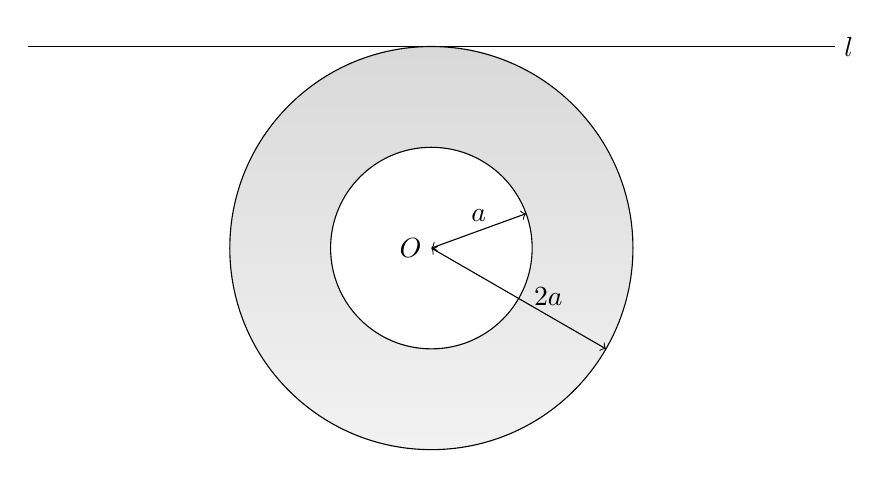
\begin{tikzpicture}[scale=0.64]
		\shadedraw[top color=gray!30,bottom color=gray!10, draw=black] (0,0) circle(4);
		\draw[fill=white] (0,0) node[left]{$O$} circle(2);
		\draw (-8,4) -- (8,4) node[right]{$l$};
		\draw[<->] (0,0) -- (20:2) node[midway,above]{$a$};
		\draw[<->] (0,0) -- (-30:4) node[pos=0.67,above]{$2a$};
		\end{tikzpicture}
		%Example \ref{ex-annulus}
	\end{center}
\end{figure}

\vspace*{-0.5\baselineskip}

apply perpendicular axis and parallel axis theorem for the full disc and the removed part\footnote{Note that the axis through $O$ parallel to $l$ lies within plane of lamina, we need to use perpendicular axis theorem to find the moment of inertia about this axis, then use parallel axis theorem to find the moment of inertia about $l$.}:

{

\centering

$I_\text{disc} = \frac{1}{2}\cdot \frac{1}{2} m(2a)^2 + m(2a)^2 = 5ma^2, \quad I_\text{removed} = \frac{1}{2}\cdot \frac{1}{2}\frac{m}{4}a^2 + \frac{m}{4}(2a)^2 = \frac{17}{16}ma^2$

$I = I_\text{disc} - I_\text{removed} = 5ma^2 - \frac{17}{16}ma^2 \RA I= \frac{63}{16}ma^2$

}

when displaced by $\theta$ from downward vertical, equation of motion $\tau = I \ddot{\theta} $ can be written as:

{

\centering

$ - \frac{3m}{4}g\cdot2a\sin\theta = \frac{63}{16}ma^2 \cdot \ddot{\theta} \RA \ddot{\theta} = -\frac{8g}{21a}\sin\theta$

}

apply small-angle approximation $\sin\theta\approx\theta$, we have: $\ddot{\theta} = -\frac{8g}{21a}\theta$

so the annulus describes approximate simple harmonic motion, and its period is

{
	
\centering

$T=\frac{2\pi}{\omega}=2\pi\sqrt{\frac{21a}{8g}} \RA T=\pi\sqrt{\frac{21a}{2g}}$

}

to complete full turn, the annulus must reach highest position where $O$ is vertically above $l$

consider conservation of energy: $\Delta E_k = \Delta E_p$, we have:

{
	
\centering
	
$ \frac{1}{2}I\omega_0^2 - \frac{1}{2}I\omega^2 = \frac{3}{4}mg\cdot 4a \RA \omega_0^2 = \omega^2 + \frac{6mga}{I} = \omega^2 + \frac{32g}{21a} \RA \omega_0^2 \geq \frac{32g}{21a}$
	
}

minimum value of $\omega_0$ is therefore $\omega_{0,\tmin} = \frac{32g}{21a}$ \eoe

\subsection{analogy with linear motion}

\vspace*{0.5\baselineskip}

\begin{center}
	{\renewcommand{\arraystretch}{1.2}
	\renewcommand{\tabcolsep}{0.2cm}
	\begin{tabular}{|c|c|c|}
	\hline
	 & linear motion & rotational motion \\ \hline
	position & displacement $x$ & angular displacement $\theta$ \\ \hline
	state of motion & velocity $v$ & angular velocity $\omega$ \\ \hline
	change of state & acceleration $a$ & angular acceleration $\alpha$ \\ \hline
	interaction & force $F$ & torque/moment $\tau$ \\ \hline
	inertia & mass $m$ & moment of inertia $I$ \\ \hline \hline
	equation of motion & $F=ma$ & $\tau = I \alpha$ \\ \hline
	kinetic energy & $E_k = \frac{1}{2}mv^2$ & $E_k = \frac{1}{2}m\omega^2$ \\ \hline
	work done & $W=Fx$ & $W=\tau \theta$ \\ \hline
	\end{tabular}}
\end{center}